\documentclass[paper=a4, fontsize=11pt]{scrartcl}
\usepackage[T1]{fontenc}
\usepackage{fourier}

\usepackage[english]{babel}                             % English language/hyphenation
\usepackage[protrusion=true,expansion=true]{microtype}  
\usepackage{amsmath,amsfonts,amsthm} % Math packages
\usepackage[pdftex]{graphicx} 
\usepackage{url}
\usepackage[section]{placeins}

%%% Custom sectioning
\usepackage{sectsty}
\allsectionsfont{\centering \normalfont\scshape}
\usepackage{color}
\usepackage{color,soul}

%%% Custom headers/footers (fancyhdr package)
\usepackage{fancyhdr}
\pagestyle{fancyplain}
\fancyhead{}                      % No page header
\fancyfoot[L]{}                     % Empty 
\fancyfoot[C]{}                     % Empty
\fancyfoot[R]{\thepage}                 % Pagenumbering
\renewcommand{\headrulewidth}{0pt}      % Remove header underlines
\renewcommand{\footrulewidth}{0pt}        % Remove footer underlines
\setlength{\headheight}{13.6pt}


%%% Equation and float numbering
\numberwithin{equation}{section}    % Equationnumbering: section.eq#
\numberwithin{figure}{section}      % Figurenumbering: section.fig#
\numberwithin{table}{section}       % Tablenumbering: section.tab#


%%% Maketitle metadata
\newcommand{\horrule}[1]{\rule{\linewidth}{#1}}   % Horizontal rule

\title{
    %\vspace{-1in}  
    \usefont{OT1}{bch}{b}{n}
    \normalfont \normalsize \textsc{Carnegie Mellon University - Computational Biology Department} \\ [25pt]
    \horrule{0.5pt} \\[0.4cm]
    \huge Active Learning for Drug Selection\\ on Identified Target Protein \\
    \horrule{2pt} \\[0.5cm]
}
\author{
  Christine Baek\\
  \normalsize\texttt{christib@andrew.cmu.edu}
  \and
  Qi Chu\\
  \normalsize\texttt{qchu@andrew.cmu.edu}
  \date{}
}
\date{}


\newcommand{\TODO}[1]{\textcolor{red}{\textbf{TODO: } #1}}

%%% Equation and float numbering
\numberwithin{equation}{section}    % Equationnumbering: section.eq#
\numberwithin{figure}{section}      % Figurenumbering: section.fig#
\numberwithin{table}{section}       % Tablenumbering: section.tab#








%%% Begin document
\begin{document}
\maketitle
\section{Introduction}
In this project, we explore three datasets of different noise level, for identification compounds, or drugs that bind to specific target protein associated with disease. We use DHM as our active learning strategy to determine when to query the Oracle, and SVM to train our model on the oracle-obtained as well as inferred labels. 



\section{Methods}

Input :
\begin{itemize}
\item Training data consists of 4000 training instances, each with 1000 features, and true label 
\item Test data consists of 1000 testing instances, each with 1000 features, and true label
\item Blind prediction data consists of 1000 instances, each with 1000 features
\end{itemize}

\TODO{discuss ~\cite{ref:warmuth}}

Based on this, we chose DHM as our base learner strategy, and SVM as our classifier, elaborated below.

\subsection{Base Learner Strategy}

DHM was chosen as our base learner strategy~\cite{ref:dhm}. DHM is a good general strategy in agnostic setting, and provides an extended version of selective sampling scheme of CAL algorithm ~\cite{ref:cal},~\cite{ref:dhm}. We compare the performance of our algorithm against random learner to test the effectiveness of the algorithm in selecting meaningful datapoints for query into the Oracle.

\TODO{talk about modifications made to the algorithm}
\subsection{Classifier Strategy}

\TODO{elaborate}


SVM was chosen as our classifier for multiple reasons. Given the high dimension of our input data (1000 features), it was important that a classifier that scales easily to high dimension, with no local optima. 
Gaussian kernel (dfault) was used for training. 


\section{Results}

\subsection{Easy}


\begin{figure}[!htb]
  \centering
  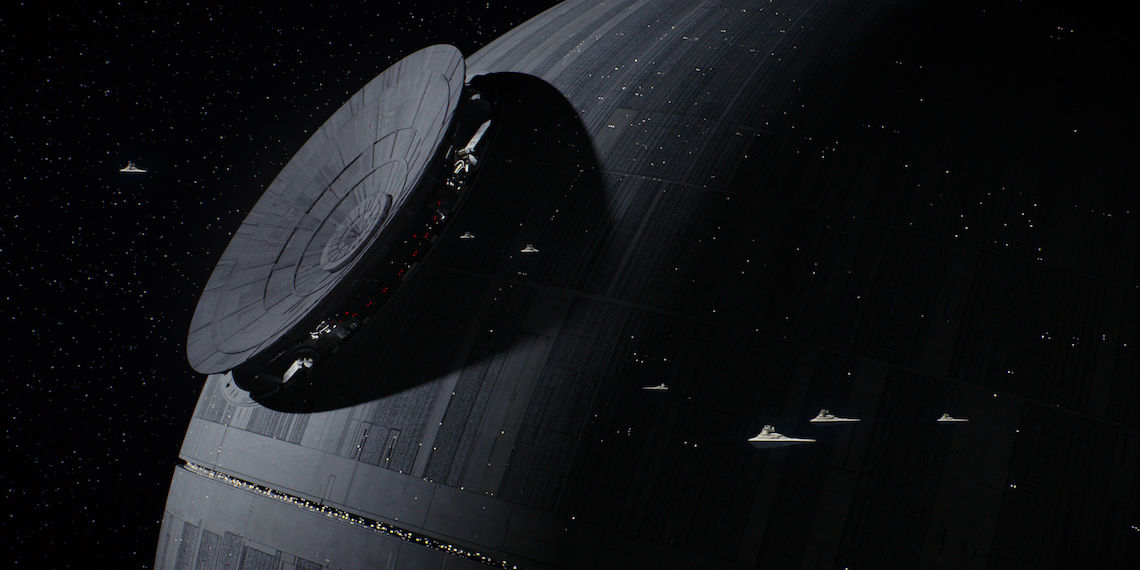
\includegraphics[scale = 0.35]{figures/fig.jpg}
      \caption{Error rate of easy test set plotted against number of queries made to oracle}
      \label{easyerror}
\end{figure}


\begin{figure}[!htb]
  \centering
  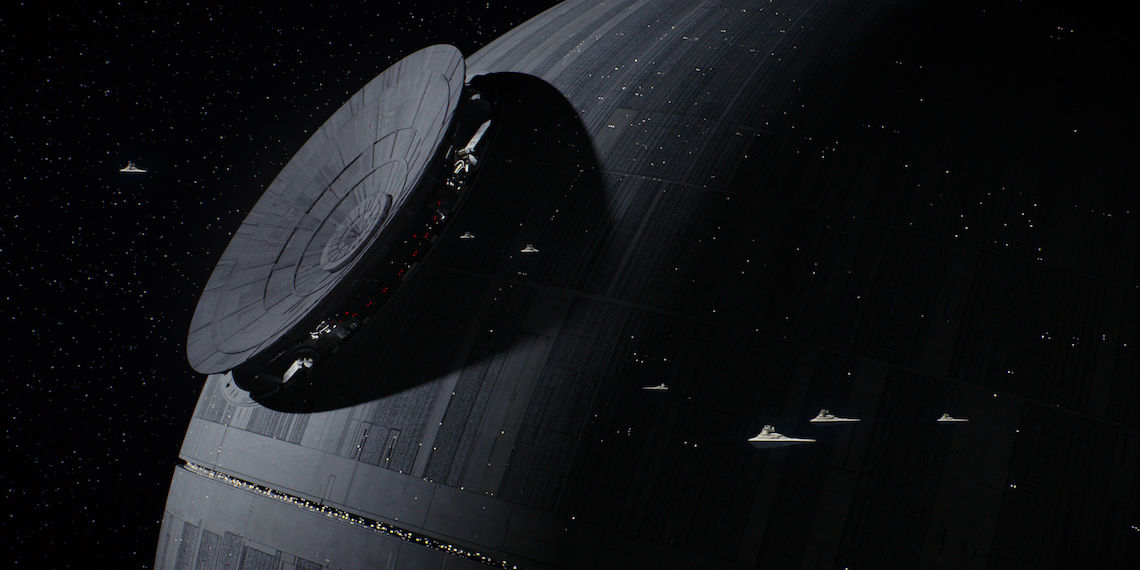
\includegraphics[scale = 0.35]{figures/fig.jpg}
      \caption{F1 Score of easy test set plotted against number of queries made to oracle}
      \label{easyf}
\end{figure}



\FloatBarrier
\subsection{Moderate}

\begin{figure}[!htb]
  \centering
  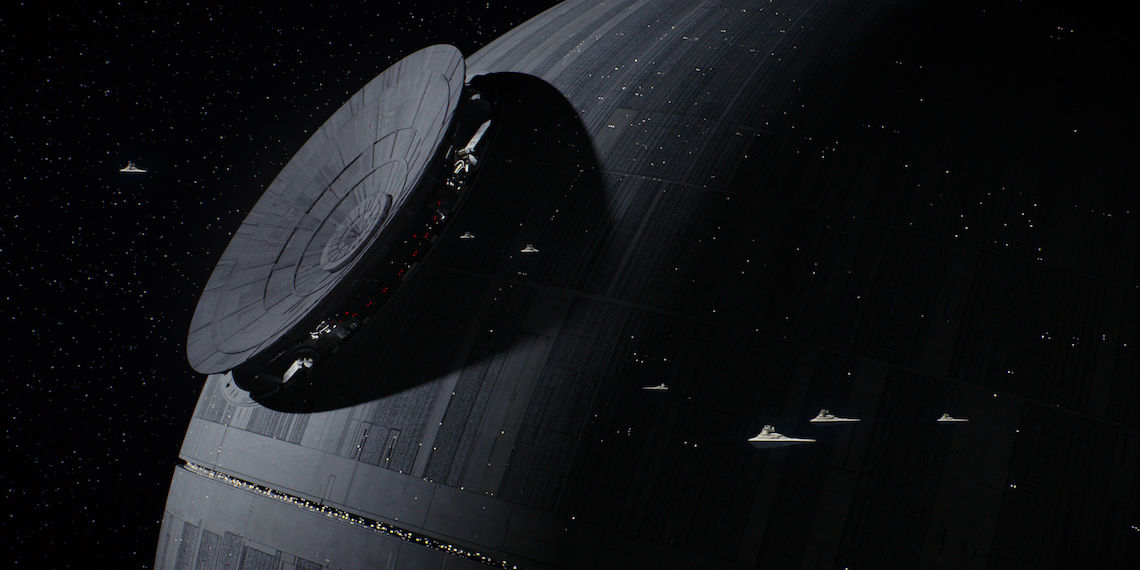
\includegraphics[scale = 0.35]{figures/fig.jpg}
      \caption{Error rate of moderate test set plotted against number of queries made to oracle}
      \label{moderror}
\end{figure}

\begin{figure}[!htb]
  \centering
  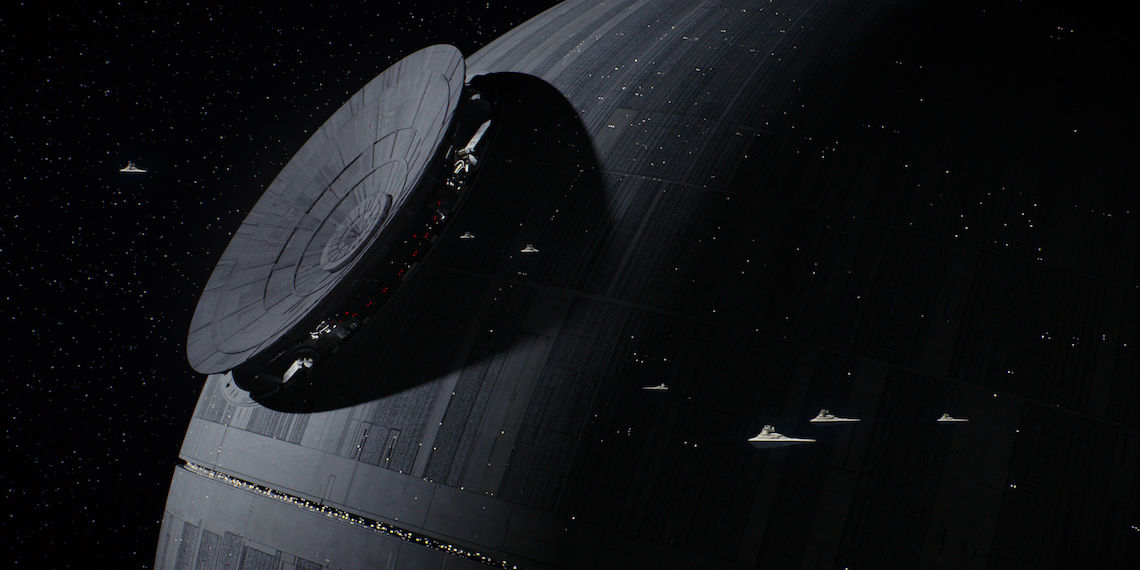
\includegraphics[scale = 0.35]{figures/fig.jpg}
      \caption{F1 score of moderate test set plotted against number of queries made to oracle}
      \label{modf}
\end{figure}
\FloatBarrier
\subsection{Difficult}


\begin{figure}[!htb]
  \centering
  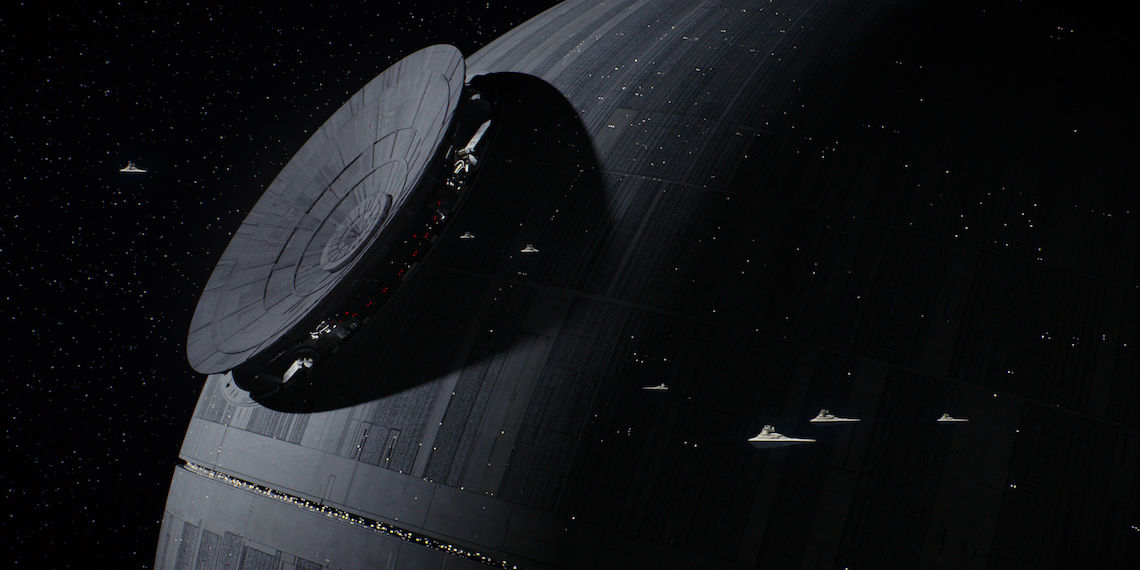
\includegraphics[scale = 0.35]{figures/fig.jpg}
      \caption{Error rate of difficult test set plotted against number of queries made to oracle}
      \label{harderror}
\end{figure}

\begin{figure}[!htb]
  \centering
  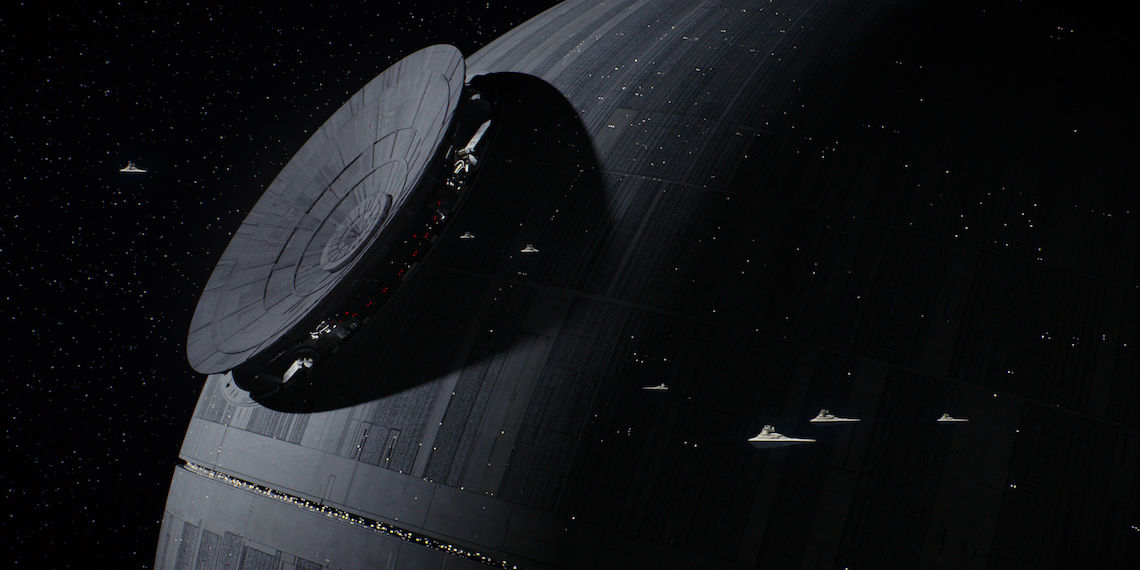
\includegraphics[scale = 0.35]{figures/fig.jpg}
      \caption{F1 score of difficult test set plotted against number of queries made to oracle}
      \label{hardf}
\end{figure}


\FloatBarrier

\section{Conclusion}

\TODO{briefly summarize}


\begin{thebibliography}{1}

\bibitem{ref:cal}
Cohn, Atlas, Ladner, \emph{Improving  Generalization  with  Active  Learning},  Machine Learning May 1994, Volume 15, Issue 2, p 201-221

\bibitem{ref:dhm}
S. Dasgupta, D. Hsu, C. Monteleoni, \emph{A general agnostic active learning algorithm}, NIPS, 2008 

\bibitem{ref:twoface}
S. Dasgupta, \emph{Two faces of active learning},  \texttt{http://cseweb.ucsd.edu/$\sim$dasgupta/papers/}, 2010

\bibitem{ref:warmuth}
Warmuth, Liao, Ratsch, Mathieson, Putta and Lemmen, \emph{Active Learning with Support Vector Machines in the Drug Discovery Process}, J. Chem. Inf. Comput. Sci. 2003, 43, 667-673

\end{thebibliography}


\end{document}